\documentclass{report}

\usepackage{listings}
\usepackage[a4paper, top=2cm, bottom=2cm, left=2cm, right=2cm]{geometry}
\usepackage{graphicx}
\usepackage{caption}
\usepackage{subcaption}
\graphicspath{ {images/} }

\title{Thema 9}
\author{Maximilian Göhring, Leander Funken}

\begin{document}

\maketitle

\section*{Info}
Alle Testergebnisse wurden auf der largemem Partition des Mogon-NHR gemessen.
\newline
Alle Ergebnisse wurden mit \verb|OMPI_MCA_btl=tcp,self| gemessen, wenn nicht 
explizit anders gesagt.
\newpage
\section*{9.1}
\subsection*{Ping-Pong}
Wir haben ein simples Ping-Pong Programm gebaut. Es funktioniert nur mit zwei 
Prozessen.
\subsubsection*{main}
\begin{lstlisting}
int main(int argc, char **argv){
    int rank, size, messageSize;
    MPI_Init(&argc, &argv);
    MPI_Comm_rank(&rank);
    MPI_Comm_size(&size);

    handle_args(argc, argv, &messageSize);

    if(rank == 0){
        root_ping_pong(messageSize);
    }else{
        node_ping_pong(messageSize);
    }

    return 0;
}
\end{lstlisting}
Zur Lesbarkeit habe ich einige Argumente und Error-handling weggelassen.
Zur Funktion:
Argumente wie messageSize werden angewendet. Dann findet der Prozess heraus 
welchen Rang er hat. Hat er Rang 0, ist er der Root-Prozess
und führt die \verb|root_ping_pong()| Funktion aus, sonst führt er die
\verb|node_ping_pong()| Funktion aus.
\subsubsection*{root}
\begin{lstlisting}
void root_ping_pong(int messageSize){
    char sendBuffer[messageSize];
    char recvBuffer[messageSize];
    generate_message(sendBuffer, messageSize);

    MPI_Send(sendBuffer);
    MPI_Recv(recvBuffer);
}
\end{lstlisting}
Der Root-Prozess sendet erst, und erhält dann eine Antwort. Die 
\verb|generate_message| Funktion
kann man im Prinzip frei wählen, für die späteren Tests haben wir den Buffer 
einfach mit "a" gefüllt um Zeit zu sparen.
Sonst wäre die Synchronisation unter Umständen gestört.
\subsubsection*{node}
\begin{lstlisting}
void node_ping_pong(int messageSize){
    char sendBuffer[messageSize];
    char recvBuffer[messageSize];
    generate_message(sendBuffer, messageSize);

    MPI_Recv(recvBuffer);
    MPI_Send(sendBuffer);
}
\end{lstlisting}
Der Node-Prozess wartet auf die Nachricht von Root und sendet dann. Abgesehen 
von der Reihenfolge ist die Funktion identisch.
\newpage
\subsection*{Ping-Exchange}
Das Ping-Exchange Programm sollte die selbe Funktion
wir Ping-Pong ausführen, aber \verb|MPI_Sendrecv()| verwenden.
Es funktioniert ebenfalls nur mit zwei Prozessen. Main:
\subsubsection*{main}
\begin{lstlisting}
int main(int argc, char **argv){
    int rank, size, messageSize;
    MPI_Init(&argc, &argv);
    MPI_Comm_rank(&rank);
    MPI_Comm_size(&size);

    handle_args(argc, argv, &messageSize);

    if(rank == 0){
        root_ping_exchange(messageSize);
    }else{
        node_ping_exchange(messageSize);
    }

    return 0;
}
\end{lstlisting}
Die main Funktion von Ping-Exchange ist identisch zu der von Ping-Pong, 
abgesehen von der root/node Funktion die aufgerufen wird.
\subsubsection*{root}
\begin{lstlisting}
void root_ping_exchange(int messageSize){
    char sendBuffer[messageSize];
    char recvBuffer[messageSize];
    generate_message(sendBuffer, messageSize);

    MPI_Sendrecv(sendBuffer, recvBuffer);
}
\end{lstlisting}
In der root Funktion wird eigentlich nur \verb|MPI_Send|/\verb|MPI_Recv| mit 
\verb|MPI_Sendrecv| ersetzt.
\subsubsection*{node}
\begin{lstlisting}
void node_ping_exchange(int messageSize){
    char sendBuffer[messageSize];
    char recvBuffer[messageSize];
    generate_message(sendBuffer, messageSize);

    MPI_Sendrecv(sendBuffer, recvBuffer);
}
\end{lstlisting}
Dadurch dass die Reihenfolge jetzt egal ist, da es nurnoch einen Aufruf gibt, 
sieht die Funktion genauso aus wie die root Funktion. In
der Realität würden natürlich noch src und dst Parameter dazukommen, die sich 
unterscheiden.
\newpage
\section*{9.2}
Hier sollten \textbf{internode} und \textbf{intranode} Kommunikation verglichen 
werden. Dazu haben wir den
gleichen Test einmal mit \newline
\verb|srun --partition <partition> -N 2 -n 2 ./test| \newline
und einmal mit \newline
\verb|srun --partition <partition> -N 1 -n 2 ./test| \newline
durchgeführt. So wurden unsere 2 Prozesse einmal auf 1, und einmal auf 2 Nodes 
ausgeführt, sodass die Kommunikation zwischen ihnen einmal inter- und
einmal intranode war. Der Test bestand darin, eine Nachricht 100 mal hin und 
her zu senden und die Half-round-trip time zu
messen. Dann haben wir den Durchschnitt der 100 Werte errechnet. Das haben wir 
für alle Nachrichtgrößen von \( 2^{0} \) bis \( 2^{20} \) Byte 5 mal gemacht.
\begin{center}
	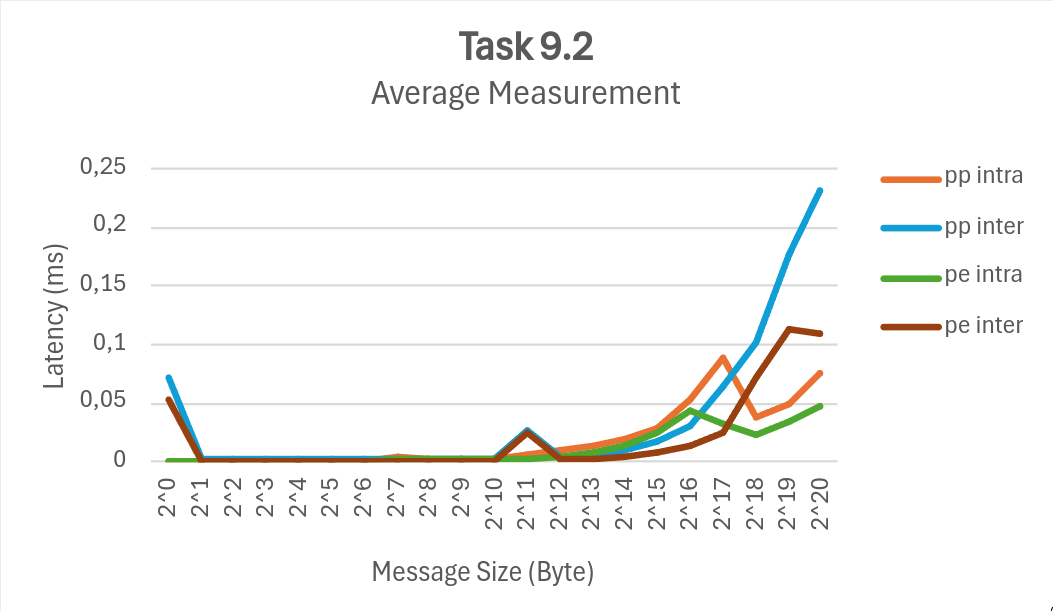
\includegraphics[width=\textwidth]{Intra-Inter}
\end{center}
Bei einer Message size von \( 2^{17} \) gab es bei all unseren 
\textbf{intranode} Messungen einen signifikanten Spike. Wir vermuten dass MPI 
kleinere Nachrichten
bei intranode Kommunikation anders behandelt als größere und ab einer Größe von 
\( 2^{17} \) umspringt, da die Performance danach schlagartig besser wird, und
sogar teilweise die Zeit von \( 2^{16} \) unterbietet. \newline
Außerdem ist aufgefallen, dass trotz der 100 Messungen pro Durchgang, der erste 
von den 5 Durchgängen bei einige Größen immer deutlich länger
dauerte als die anderen.
\newpage
\section*{9.3}
Hier sollten wir \verb|numactl --cpunodebind=(0,1)| verwenden, um bestimmte cpu 
nodes zu nutzen. Wir haben uns entschieden für klarere
Ergebnisse Messungen mit \verb|numactl --cpunodebind=(0,1,7)| durchzuführen, da 
7 die höchste node in largemem ist. Anfangs schienen diese
Daten eindeutig zu sein. Nachdem wir für andere Messungen immer mehr äußere 
Einflüsse, wie zum Beispiel zufällige Nachrichtengenerierung, entfernt
haben, haben sich die Ergebnisse jedoch immer weiter angegleicht.
\begin{figure}[h]
	\begin{subfigure}{.5\textwidth}
		\centering
		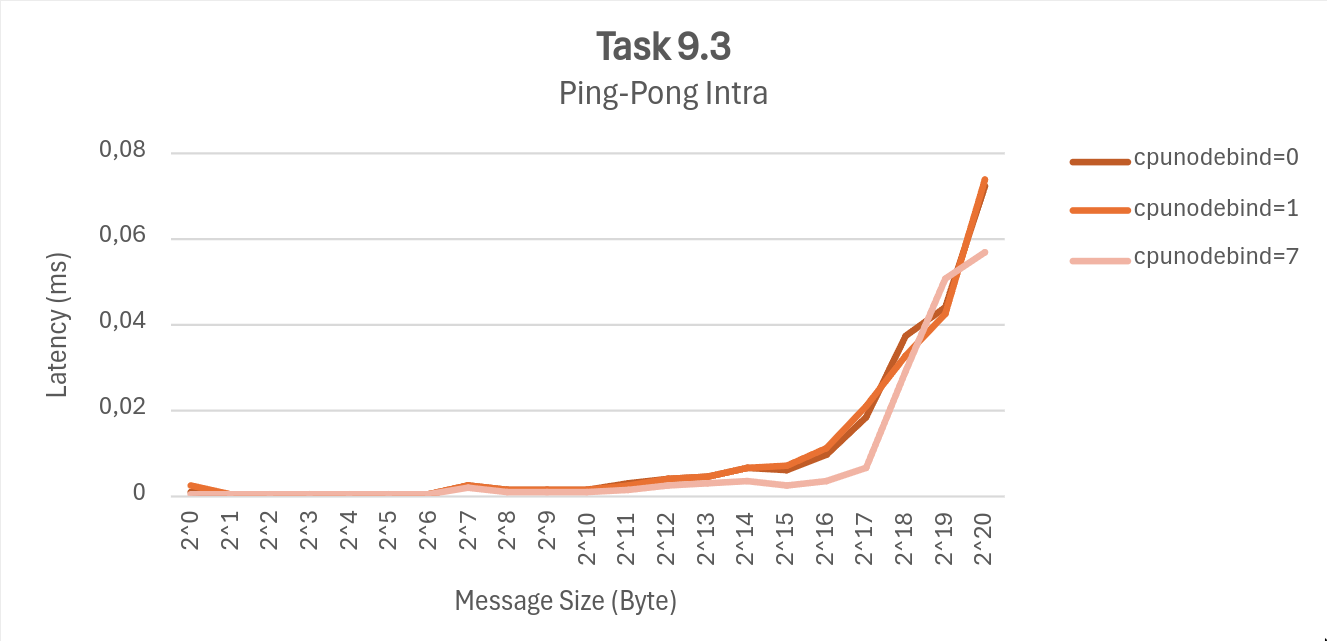
\includegraphics[width=\textwidth]{cpunodebind0}
	\end{subfigure}
	\begin{subfigure}{.5\textwidth}
		\centering
		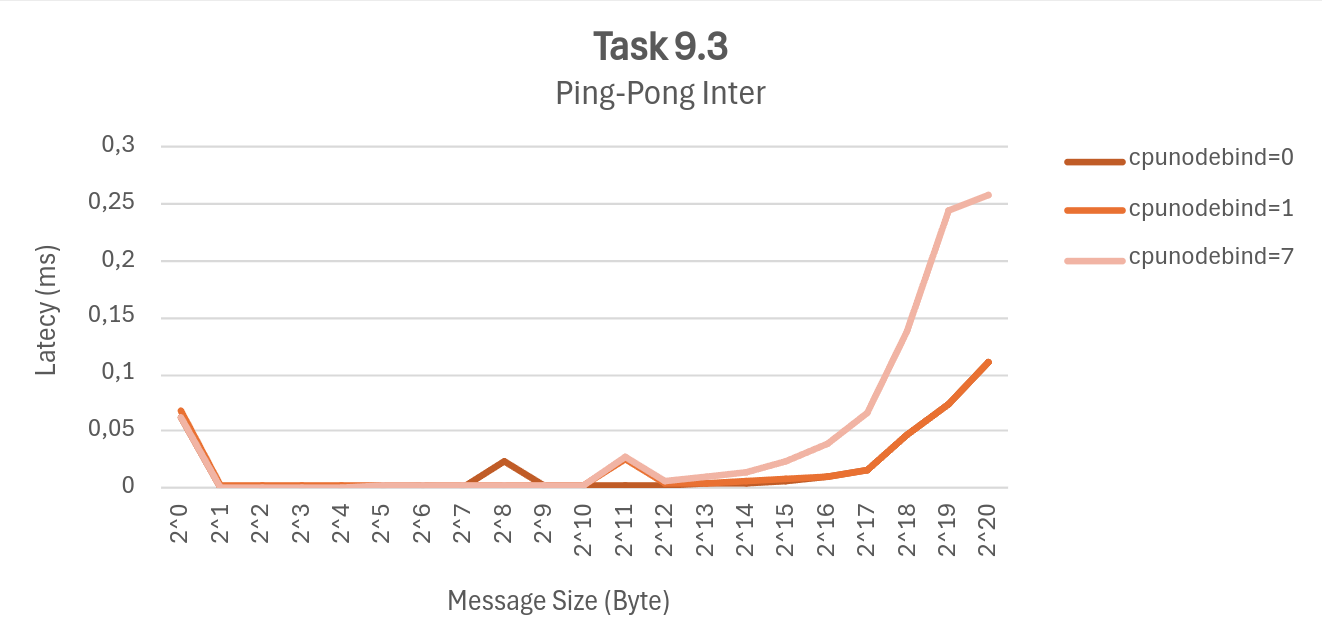
\includegraphics[width=\textwidth]{cpunodebind1}
	\end{subfigure}
\end{figure}
\begin{figure}[h]
	\begin{subfigure}{.5\textwidth}
		\centering
		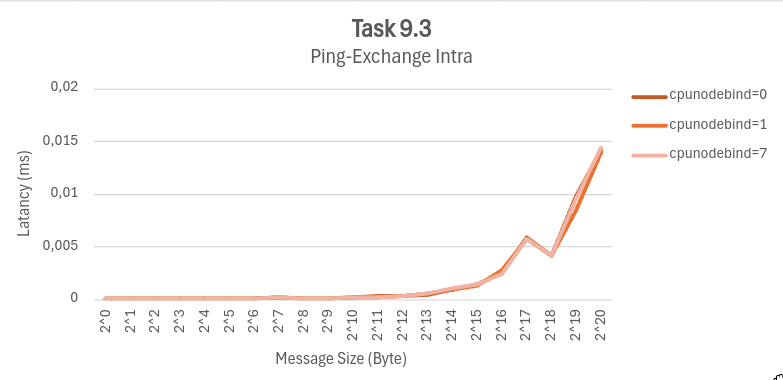
\includegraphics[width=\textwidth]{cpunodebind2}
	\end{subfigure}
	\begin{subfigure}{.5\textwidth}
		\centering
		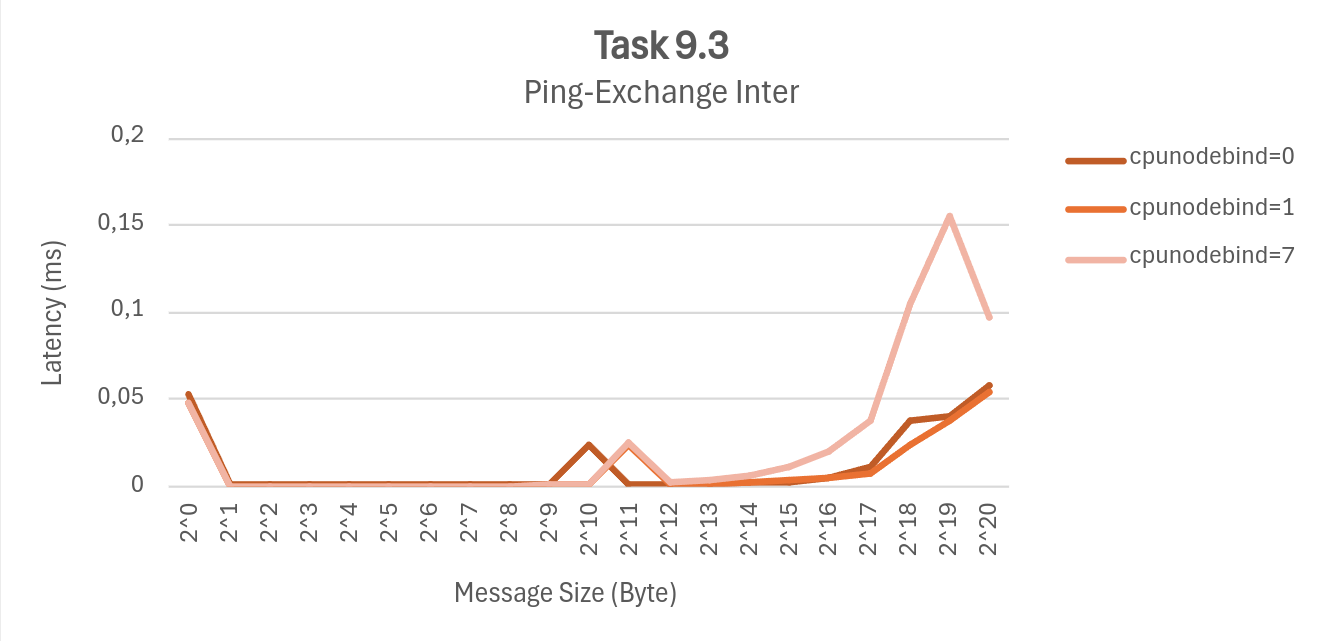
\includegraphics[width=\textwidth]{cpunodebind3}
	\end{subfigure}
\end{figure}
\end{document}
